% \section{01 section}
% \label{sec:01label}

%% Template
\subsection{Frequency Domain Analysis}
\begin{frame} \frametitle{Frequency Domain Analysis}
    \framesubtitle{FSK Modulation and Fourier Transformation}
    \begin{block}{Satelite Simulation and Recordings}    
        \begin{center}
            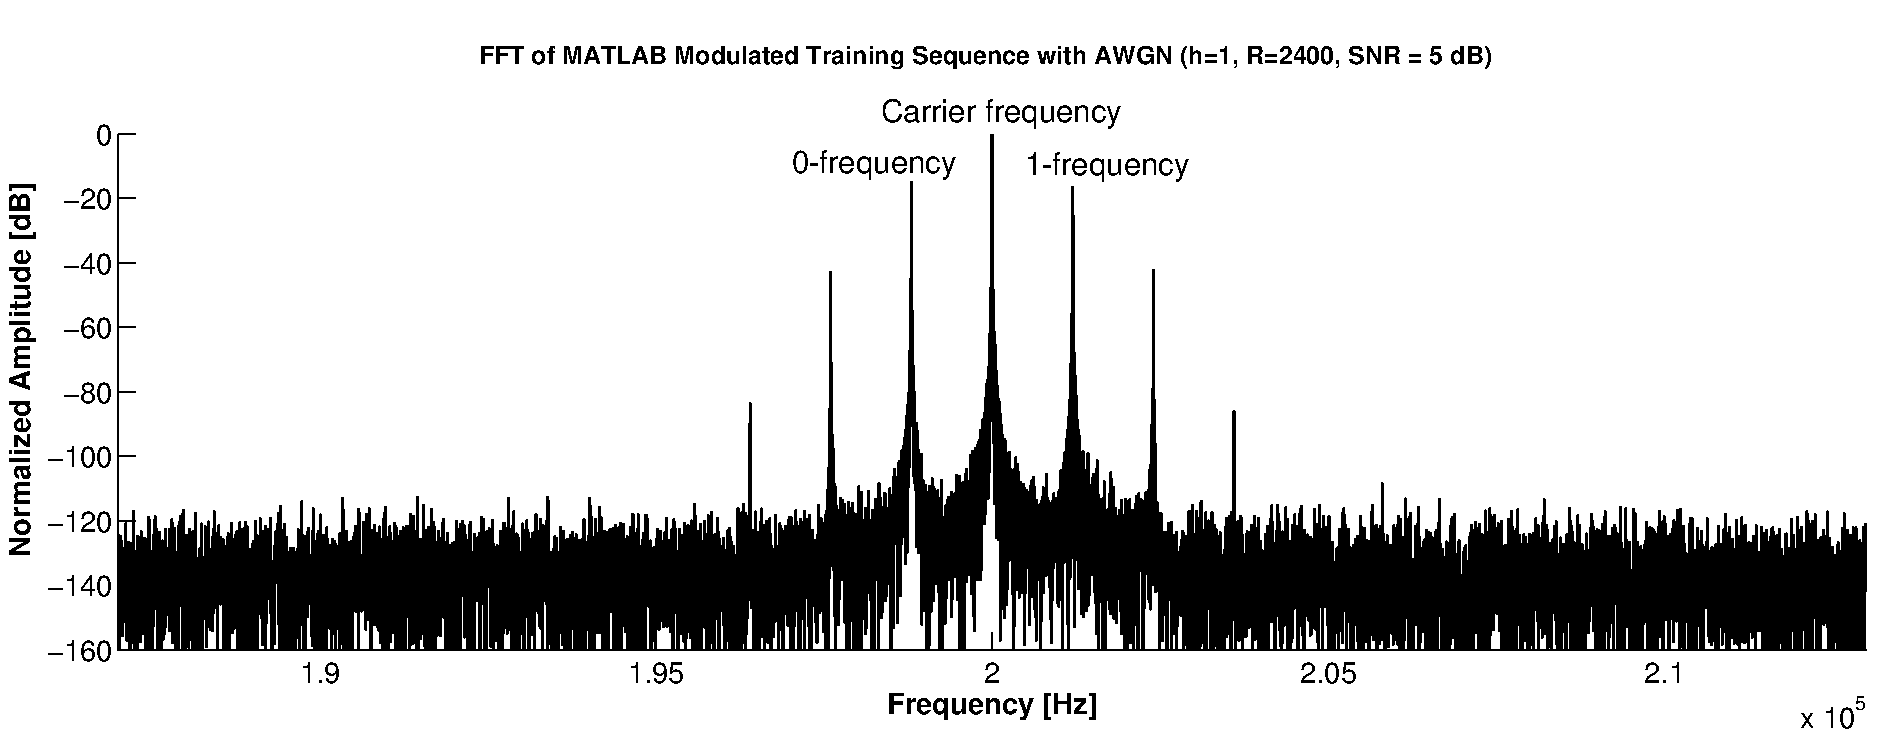
\includegraphics[width=0.8\textwidth]{img/fft_train_seq}
        \end{center}
        \begin{center}
            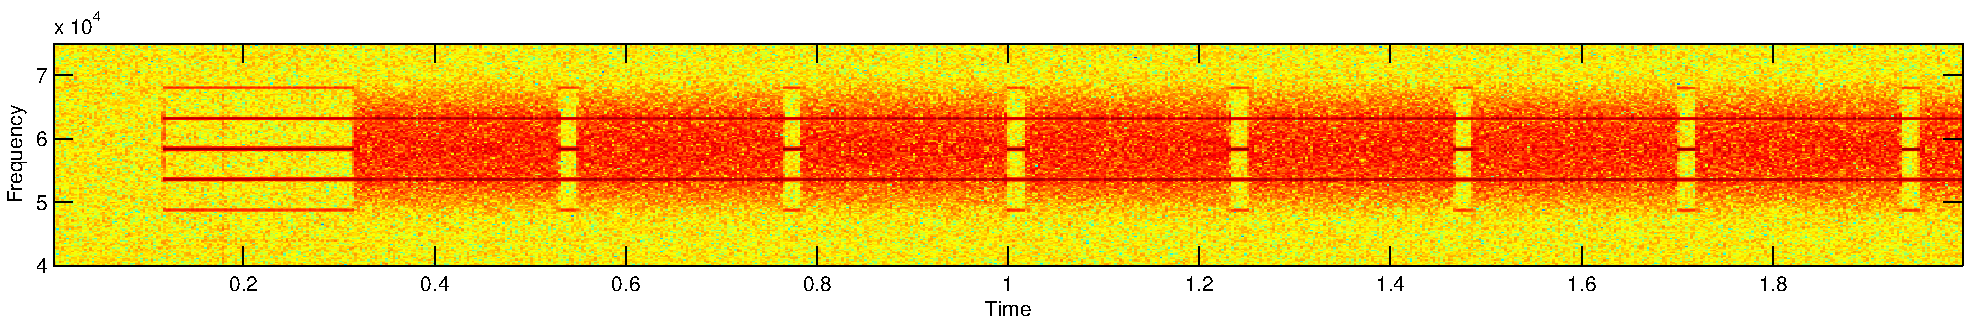
\includegraphics[width=0.8\textwidth]{img/packet_from_recording}
        \end{center}
        \begin{itemize}
            \item Estimating carrier frequency.
            \item Errors at low frequency in windmill.
            \item Estimation of noise.
        \end{itemize}
    \end{block}
\end{frame}

\subsection{Filter Design}
\begin{frame} \frametitle{Filter Design}
    \begin{block}{Filter Design Specs}    
        \begin{center}
            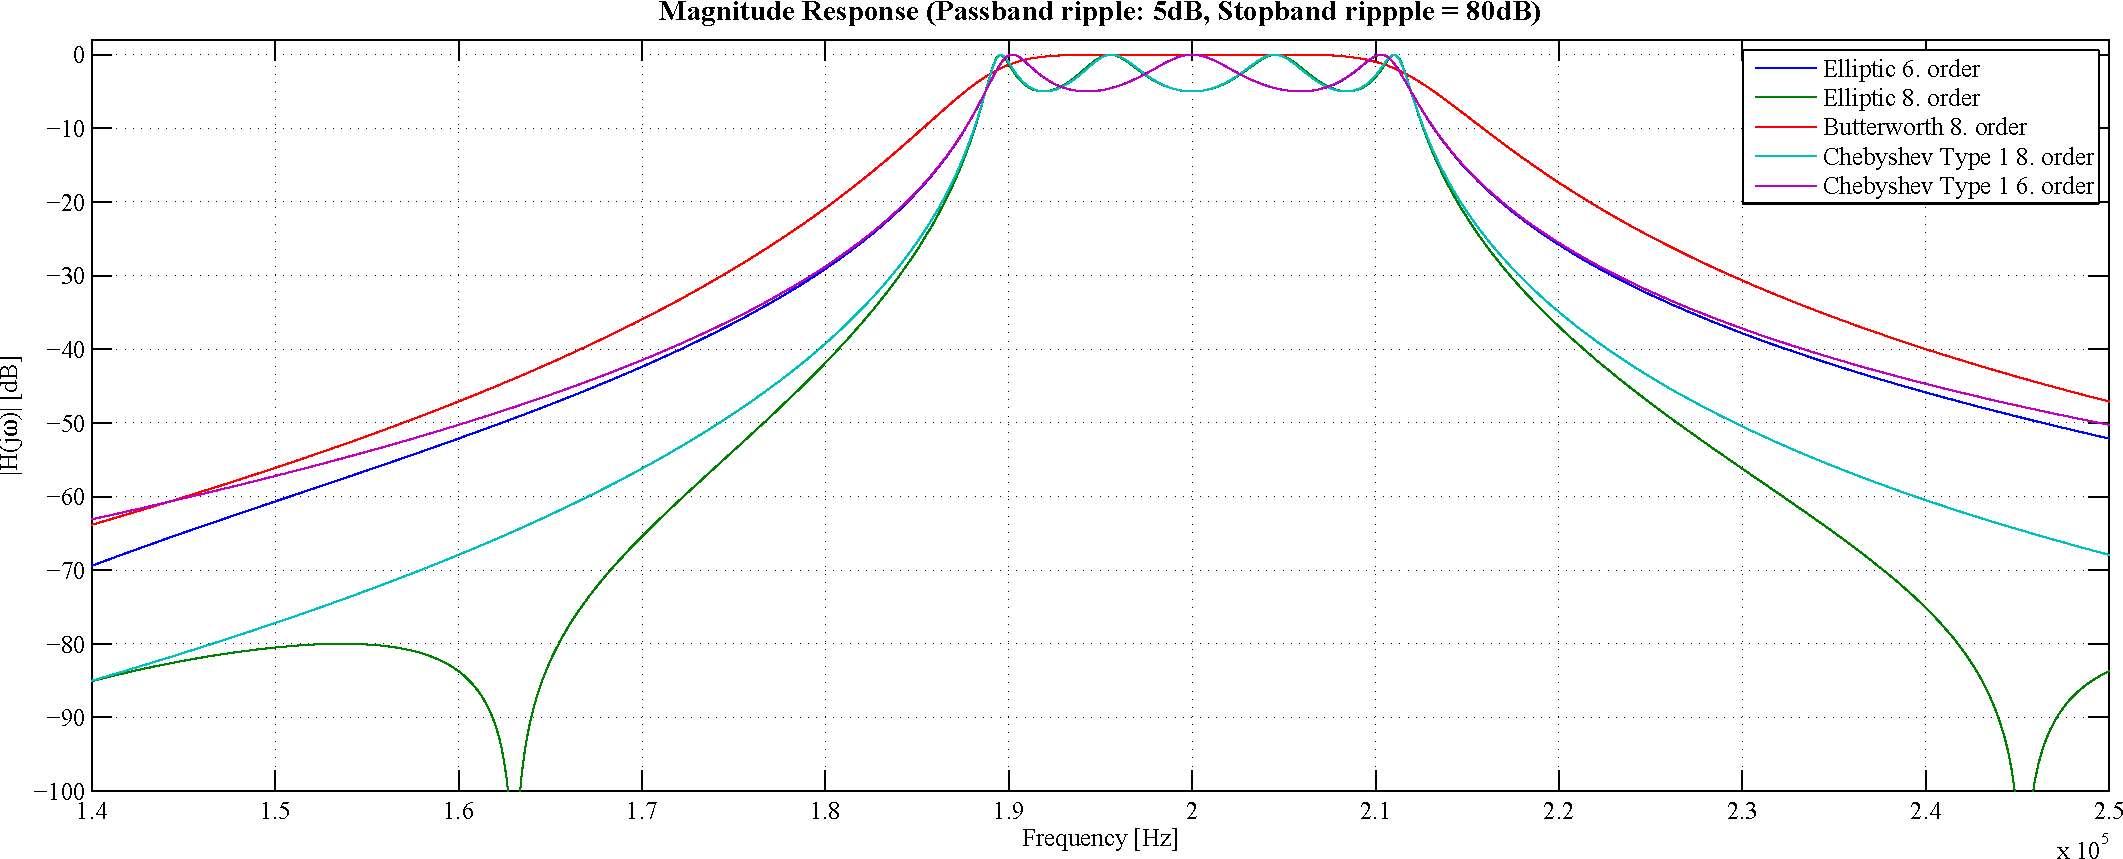
\includegraphics[width=0.8\textwidth]{img/filter2_frq_res}
        \end{center}
        \begin{itemize}
            \item Doppler Shift Range.
            \item Speech Area.
        \end{itemize}
    \end{block}
\end{frame}

\subsection{Filter Implementation}
\begin{frame} \frametitle{Filter Implementation}
    \framesubtitle{From $s$-domain to $z$-domain}
    \begin{block}{Filter Design Specs}    
        \begin{center}
            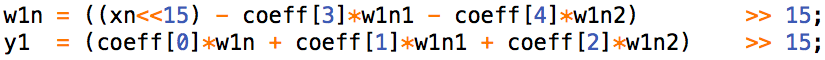
\includegraphics[width=0.8\textwidth]{img/filter_C_cascade}
        \end{center}
        \begin{center}
            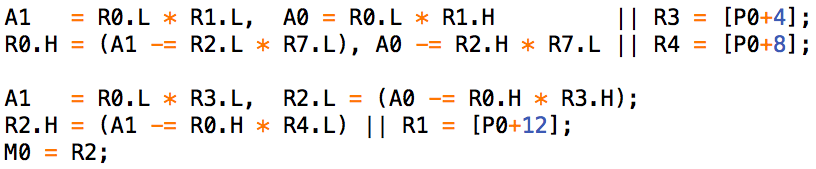
\includegraphics[width=0.8\textwidth]{img/filter_asm_cascade}
        \end{center}
        \begin{itemize}
            \item Implementing in C and ASM ($z$-domain).
        \end{itemize}
    \end{block}
\end{frame}

\subsection{Power Detection}
\begin{frame} \frametitle{Power Detection}
    \framesubtitle{Packet Detection for SDR}
    \begin{block}{Packet Detection \& Time Synchronization}    
        \begin{center}
            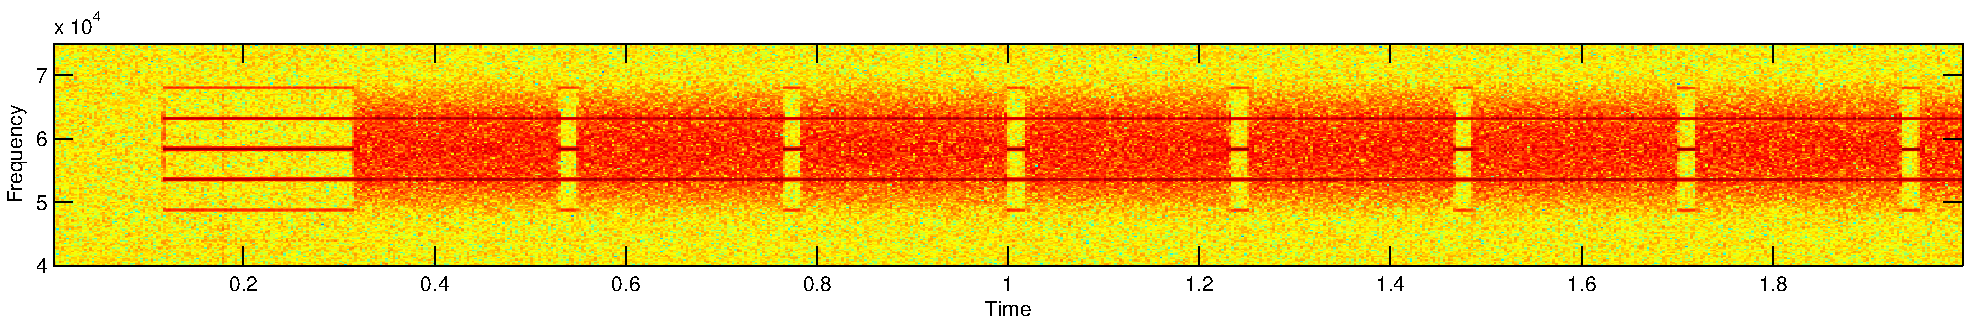
\includegraphics[width=0.8\textwidth]{img/packet_from_recording}
        \end{center}
        \begin{center}
            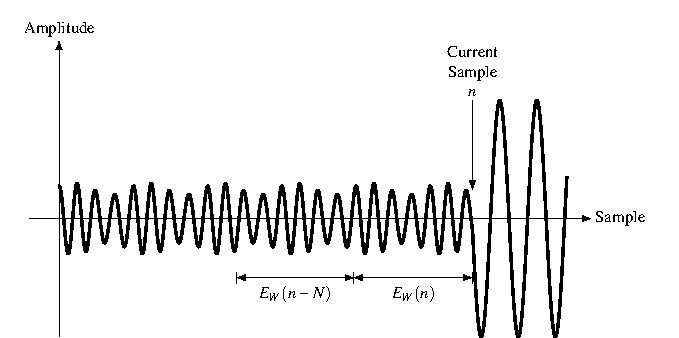
\includegraphics[width=0.8\textwidth]{img/dsw4} 
        \end{center}
        \begin{itemize}
            \item Could also be for localization of speech.
        \end{itemize}
    \end{block}
\end{frame}

\subsection{Results}
\begin{frame} \frametitle{System Output}
    \framesubtitle{Analog to Binary format}
    \begin{block}{FSK - Frequency Shift Keying}    
        \begin{center}
            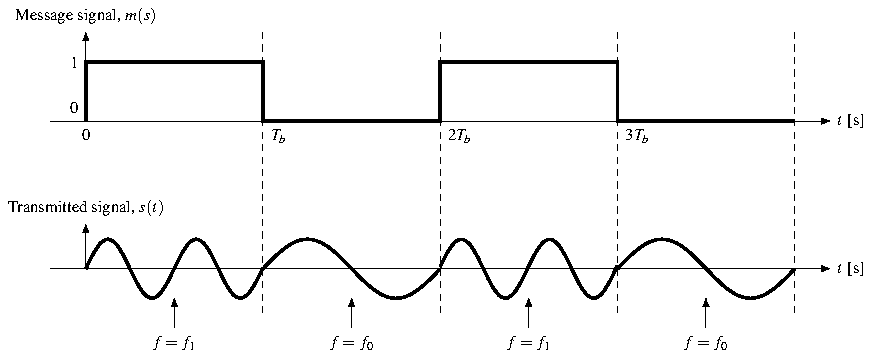
\includegraphics[width=0.8\textwidth]{img/gfsk_basics}
        \end{center}
        \begin{itemize}
            \item $f_0$ and $f_1$.
        \end{itemize}
    \end{block}
\end{frame}
%
\begin{frame}\frametitle{System Output}
    \begin{block}{Phase input to Binary Output} 
        \begin{center}
            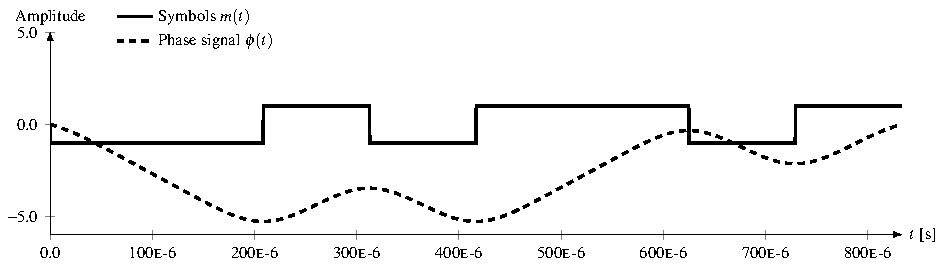
\includegraphics[width=0.8\textwidth]{img/gfsk_integration} 
        \end{center}
        \begin{equation}
            \phi(t) = \phi(0) + \frac{h \pi}{T_b}\int_0^{T_b} m_{NRZ}dt
        \end{equation}
    \end{block}
\end{frame}


\begin{frame}\frametitle{Related Masters}
    \begin{block}{Within Signal Processing} 
     \begin{itemize}
         \item Signal Processing and Computing.
         \item Acoustics
         \item Sound \& Music Computing.
     \end{itemize}
    \end{block}
\end{frame}

